\section{Analysis}\label{sec:Analysis}

\subsection{Data preparation}

As the initial step of the analysis the data is prepared.
First all Monte-Carlo truths, event identification numbers and weights are removed so that only the simulated measurements and
event-labels which will later be used for supervised learning are left. In the next step all simulated measurement with missing or
infinite values are removed from the data. Furthermore all columns that contain te same value in every line are deleted.
Finally in both the simulated signal- and backgrounddata attributes which are not contained in the other are removed und
both datasets are combined to one. \\
Finally the data is split in a test- and training-dataset while $80 \, \%$ of the data is used for training and $20 \,\%$
for testing.

\subsection{Forward selection}

In the next step of the analysis the number of features is reduced by determining the most important features using
the \texttt{SelectKBest} with \texttt{$f_classif$} from the \texttt{sklearn} library and removing all other features. \\
For this the dataset is sequentially reduced to $N \in \{ 10, \, 20, \, 30, \, 40, \, 40, \, 50, \, 60, \, 70, \, 80, \, 90, \, 100 \}$
features and for each number of features the jaccard index is determined for the Naive-Bayes Classifier \texttt{GaussianNB}.
In the end the number of features that yields the highest jaccard index is selected for the analysis.
In the run used for the analysis the best jaccard index was archieved for $50$ features. \\
The best $50$ features are determined using \texttt{SelectKBest} and all other features are removed from the data.

\subsection{The classifiers}

For the seperation of the singal data from the background data the classifiers $\texttt{RandomForestClassifier}$, $\texttt{KNeighborsClassifier}$
and $\texttt{GaussianNB}$ from $\texttt{sklearn}$ are used. in the case of $\texttt{RandomForestClassifier}$ and  $\texttt{KNeighborsClassifier}$
the optimal number of trees and neighbours is determined analogously to the number of attributes by trying different values and choosing
the value with the largest jaccard index. The optimal values are $N_\text{trees} = 140$ and $N_\text{neighbours} = 90$.\\
All classifiers are trained on the training data and the jaccard index, purity and efficiency are determined with crossvalidation.
The values are listed in table \ref{tab:results}. \\
Finally a receiver operating characteristic is generated and pictured in figure \ref{fig:ROC}.

\begin{figure}[tb]
  \centering
  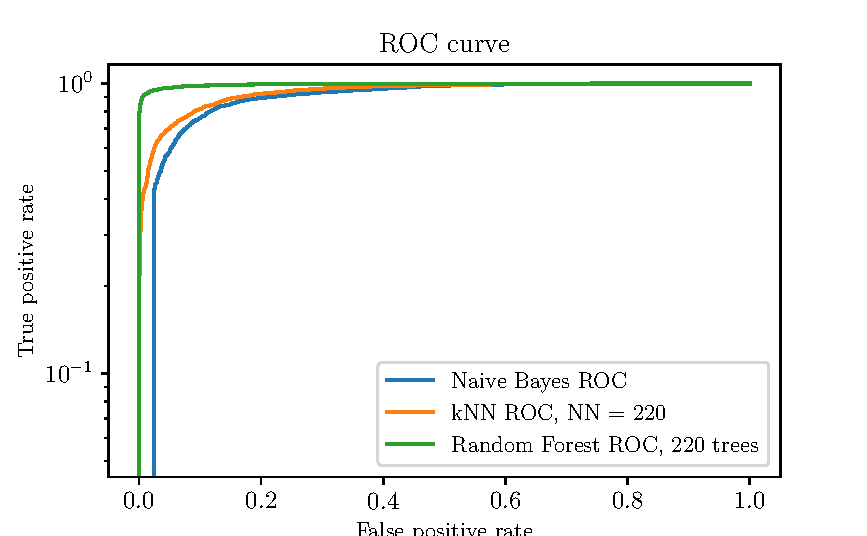
\includegraphics[width=12cm,keepaspectratio]{plots/ROC.pdf}
  \caption{ROC curves for the three differrent classifiers.}
  \label{fig:ROC}
\end{figure}

\begin{table}
  \centering
  \begin{tabular}{c | c c c}
    \toprule
    \text{Classifier} & \text{Efficiency} & \text{Purity} & \text{Jaccard index} \\
    \midrule
    \text{RandomForest} & $\num{0.9530 \pm  0.0093}$ & $\num{0.9654 \pm 0.0826}$ & $\num{0.9204 \pm 0.0710}$ \\
    \text{KNeighborsClassifier} & $\num{0.8540 \pm 0.0215}$ & $\num{0.7661 \pm 0.0621}$ & $\num{0.6769 \pm 0.0407}$ \\
    \text{Naive-Bayes} & $\num{0.7970 \pm 0.0528}$ & $\num{0.7980 \pm 0.0662}$ & $\num{0.6618 \pm 0.0212}$ \\
    \bottomrule
  \end{tabular}
  \caption{Efficiency, purity and Jaccard index of the three classifiers applied to the data set.}
  \label{tab:results}
\end{table}
